\pdfminorversion=4
\documentclass[mathserif,xcolor={dvipsnames,table}]{beamer}
\mode<presentation>{\usetheme{Warsaw}\usecolortheme{crane}}
\usepackage{centernot}
\usepackage{graphicx}
\usepackage{geometry}
\usepackage{tikz}
\usetikzlibrary{shadows}
\usepackage{hyperref}
\usepackage[utf8]{inputenc}
\usepackage[english]{babel}
\usepackage[T1]{fontenc}
\usepackage{lmodern}
\usepackage[babel=true]{microtype}
\usepackage{amsmath}
\beamertemplatenavigationsymbolsempty

\title{UNIX Weapons School---The x86}
\date{}
\author{Nick Black for the\\
Georgia Institute of Technology
}

\begin{document}

\begin{frame}
\titlepage
\begin{center}

\includegraphics[scale=0.33]{images/uws.png}\\
\vspace{.1in}
\tiny{copyright \copyright\ 2013}\\

\includegraphics[scale=.25]{images/cc-logo.pdf}

\includegraphics[scale=.25]{images/cc-new.pdf}

\includegraphics[scale=.25]{images/cc-share.pdf}\\
\tiny{creative commons 3.0 share-alike attribution license}
\end{center}
\end{frame}

\begin{frame}{Why study the x86?}
The answer is not ``elegance''.
\vfill
\begin{itemize}
\item Used in a majority of servers, workstations, and laptops
\item Receives the most focus in the kernel/toolchain
\item Very complex processor, thus large optimization space
\item Excellent documentation and literature
\item Fascinating, revealing, lengthy history
\end{itemize}
\vfill
Please do not think that x86 has been all that's gone on over the past
twenty years. That said, if you can chase peak on x86, you can
probably hack on anything.
\end{frame}

\begin{frame}{Other ISAs worth knowing (about)}
\begin{columns}
\begin{column}{.5\textwidth}
\footnotesize{
\begin{itemize}
\item Alpha
\item AVR32
\item PA-RISC + MAX-2
\item SuperH 
\item i960
\item IA64 (Itanium)
\item MIPS + MIPS-3D
\item IBMHLA (s390 + z)
\item m68k
\item z80
\item VAX
\item MIX
\end{itemize}
}
\end{column}
\begin{column}{.5\textwidth}
\footnotesize{
\begin{itemize}
\item SPARC V9 + VIS3\footnote{\tiny{Most recently the ``Oracle SPARC Architecture 2011''.}}
\item JVM\footnote{\tiny{Most recently the Java SE 7 spec, 2013-02-28.}}
\item PTX/SASS\footnote{\tiny{Most recently the PTX ISA 3.1 spec, 2012-09-13.}}
\item ARM + NEON\footnote{\tiny{ARMv8: A64, A32, and T32, 2011-10-27.}}
\item Blackfin
\item PowerISA + AltiVec/VSX\footnote{\tiny{PowerISA v.2.06B, 2010-11-03.}}
\item MMIX
\end{itemize}
}
\end{column}
\end{columns}
\end{frame}


\begin{frame}[t]{IA-16 CISC (MS-DOS, 640K--1M RAM)}
\begin{block}{8086/80186 (NEC, AMD, Fujitsu, OKI, Kvazar-Mikro, \ldots)}
\begin{itemize}
\item IBM PC/XT. Real mode. 16-bit regs and buses
\item 1MB RAM in 16 64K segments
\item 8086-2 ISA on 80186
{\footnotesize
(\tt{ENTER}/\tt{LEAVE}, \tt{PUSHA}/\tt{POPA}, \tt{INS}/\tt{OUTS})
}
\end{itemize}
\end{block}
\begin{block}{80286 (IBM, AMD, Fujitsu, \ldots)}
\begin{itemize}
\item IBM PC/AT (ISA). Protected mode w/ MMU
\item 16MB RAM with privilege levels on segments
\end{itemize}
\end{block}
\vfill
\begin{center}
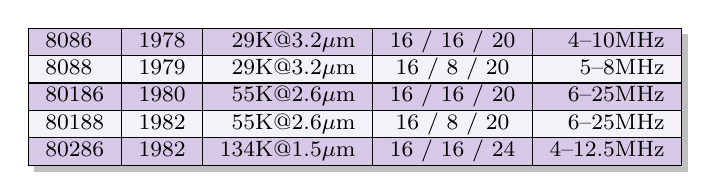
\begin{tikzpicture}
\node[drop shadow,fill=white,inner sep=0pt]
{\rowcolors{1}{RoyalPurple!20}{RoyalPurple!5}
{\footnotesize
\begin{tabular}{|l|r|r|c|r|}
\hline
8086 & 1978 & 29K@3.2$\mu$m & 16 / 16 / 20 & 4--10MHz \\
\hline
8088 & 1979 & 29K@3.2$\mu$m & 16 / 8 / 20 & 5--8MHz \\
\hline
80186 & 1980 & 55K@2.6$\mu$m & 16 / 16 / 20 & 6--25MHz \\
\hline
80188 & 1982 & 55K@2.6$\mu$m & 16 / 8 / 20 & 6--25MHz \\
\hline
80286 & 1982 & 134K@1.5$\mu$m & 16 / 16 / 24 & 4--12.5MHz \\
\hline
\end{tabular}%
}
};
\end{tikzpicture}
\end{center}
\end{frame}

\begin{frame}[t]{IA-32 CISC (Win 3.11, OS/2, Linux, 386BSD)}
\begin{block}{80386 (Am386, TI, Chips, IBM, \ldots)}
\begin{itemize}
\item IBM PS/2 (MCA). 32-bit segments, regs, buses
\item NatSemi 16550A UART. 80386SL: first (external) cache
\item 2\textbf{c} per simple instruction
\end{itemize}
\end{block}
\begin{block}{80486 (Am486, Cx486DLC, TI486SXL, IBM486DLC,\ldots)}
\begin{itemize}
\item EISA/VLB. On-die cache, \texttt{XADD}, \texttt{CMPXCHG}
\item 1\textbf{c} per simple instruction, integrated FPU
\end{itemize}
\end{block}
\vfill
\begin{center}
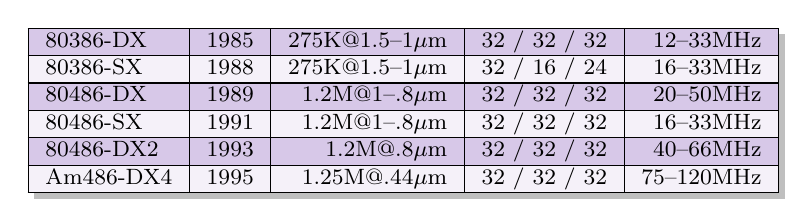
\begin{tikzpicture}
\node[drop shadow,fill=white,inner sep=0pt]
{\rowcolors{1}{RoyalPurple!20}{RoyalPurple!5}
{\footnotesize
\begin{tabular}{|l|r|r|c|r|}
\hline
80386-DX & 1985 & 275K@1.5--1$\mu$m & 32 / 32 / 32 & 12--33MHz \\
\hline
80386-SX & 1988 & 275K@1.5--1$\mu$m & 32 / 16 / 24 & 16--33MHz \\
\hline
80486-DX & 1989 & 1.2M@1--.8$\mu$m & 32 / 32 / 32 & 20--50MHz \\
\hline
80486-SX & 1991 & 1.2M@1--.8$\mu$m & 32 / 32 / 32 & 16--33MHz \\
\hline
80486-DX2 & 1993 & 1.2M@.8$\mu$m & 32 / 32 / 32 & 40--66MHz \\
\hline
Am486-DX4 & 1995 & 1.25M@.44$\mu$m & 32 / 32 / 32 & 75--120MHz \\
\hline
\end{tabular}%
}
};
\end{tikzpicture}
\end{center}
\end{frame}

\begin{frame}[t]{Pipelined superscalar (Win 95, BeOS, FreeBSD)}
\begin{block}{Intel P5 (Pentium, Pentium MMX)}
\begin{itemize}
\item U/V pipes, I\$/D\$ split, better FPU/MUL, debug regs
\item PMMX adds MMX + performance counters (\texttt{RDPMC})
\end{itemize}
\end{block}
\begin{block}{AMD K5 (SSA/5, 5k86)}
\begin{itemize}
\item RISC Am29000 with x86 frontend emitting $\mu$code
\item Variable register window sizes
\end{itemize}
\end{block}
\begin{block}{Cyrix 6x86}
\begin{itemize}
\item Scratchpad (``L0'') cache, great ZOPS, crap FPU
\end{itemize}
\end{block}
\vfill
\begin{center}
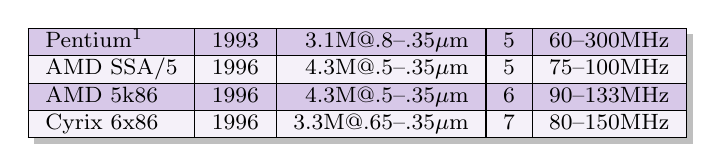
\begin{tikzpicture}
\node[drop shadow,fill=white,inner sep=0pt]
{\rowcolors{1}{RoyalPurple!20}{RoyalPurple!5}
{\footnotesize
\begin{tabular}{|l|r|r|c|r|}
\hline
Pentium\footnote{\tiny{The faster .35$\mu$m Pentiums (P54CS, P55C, Tillamook) didn't emerge until 1995 (P54CS) or 1997.}} & 1993 & 3.1M@.8--.35$\mu$m & 5 & 60--300MHz \\
\hline
AMD SSA/5 & 1996 & 4.3M@.5--.35$\mu$m & 5 & 75--100MHz \\
\hline
AMD 5k86 & 1996 & 4.3M@.5--.35$\mu$m & 6 & 90--133MHz \\
\hline
Cyrix 6x86 & 1996 & 3.3M@.65--.35$\mu$m & 7 & 80--150MHz \\
\hline
\end{tabular}%
}
};
\end{tikzpicture}
\end{center}
\end{frame}

\begin{frame}[t]{SSE + OOO CRISC (Win 98, FreeBSD 3, Linux 2)}

\begin{block}{Intel P6 (PPro / PII / PIII)}
\begin{itemize}
\item PPro adds \texttt{SYSENTER, SYSEXIT}
\item PIII adds 8 128-bit regs, SSE1 and \texttt{CMOVcc}
%SSE1 is strictly 32x4 FP + data-movement stuff, plus SFENCE
%PIII shared execution resources (save regs) between SSE/FP
\item FIXME
\end{itemize}
\end{block}
\begin{block}{AMD K6 (K6 / K6-2 / K6-III)}
\begin{itemize}
\item Adds \texttt{SYSCALL, SYSRET}
\item K6-2 adds 3DNow! atop MMX regs
% shit for performance, but worked without OS support, but who cares?
\item FIXME
\end{itemize}
\end{block}
\vfill
\begin{center}
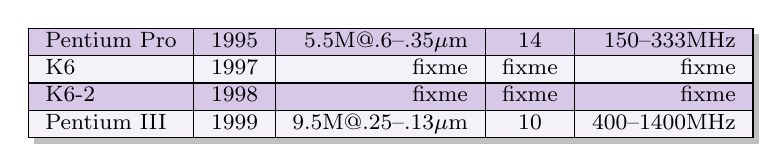
\begin{tikzpicture}
\node[drop shadow,fill=white,inner sep=0pt]
{\rowcolors{1}{RoyalPurple!20}{RoyalPurple!5}
{\footnotesize
\begin{tabular}{|l|r|r|c|r|}
\hline
Pentium Pro & 1995 & 5.5M@.6--.35$\mu$m & 14 & 150--333MHz \\
\hline
K6 & 1997 & fixme & fixme & fixme \\
\hline
K6-2 & 1998 & fixme & fixme & fixme \\
\hline
Pentium III & 1999 & 9.5M@.25--.13$\mu$m & 10 & 400--1400MHz \\
\hline
\end{tabular}%
}
};
\end{tikzpicture}
\end{center}
\end{frame}

\begin{frame}[t]{SSE2 + long pipelines (FreeBSD 4, Linux 2.4)}
\begin{block}{Intel NetBurst (P4, PD)}
\begin{itemize}
\item P4 adds SSE2, HyperThreading
% SSE2 implements MMX integer ops and 64-bit double FP
\item FIXME
\end{itemize}
\end{block}
\begin{block}{AMD K7 (Athlon)}
\begin{itemize}
\item Alpha's EV6, 3-way FPU
\item SSE2 on Palomino
\item FIXME
\end{itemize}
\end{block}
\vfill
\begin{center}
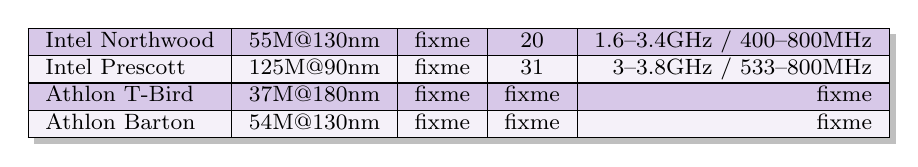
\begin{tikzpicture}
\node[drop shadow,fill=white,inner sep=0pt]
{\rowcolors{1}{RoyalPurple!20}{RoyalPurple!5}
{\footnotesize
\begin{tabular}{|l|r|r|c|r|}
\hline
Intel Northwood & 55M@130nm & fixme & 20 & 1.6--3.4GHz / 400--800MHz \\
\hline
Intel Prescott & 125M@90nm & fixme & 31 & 3--3.8GHz / 533--800MHz \\
\hline
Athlon T-Bird & 37M@180nm & fixme & fixme & fixme \\
\hline
Athlon Barton & 54M@130nm & fixme & fixme & fixme \\
\hline
\end{tabular}%
}
};
\end{tikzpicture}
\end{center}
\end{frame}

\begin{frame}[t]{IA-64 multicore (FreeBSD 7, Linux 2.6)}
\begin{block}{Intel Core}
\begin{itemize}
\item FIXME
\end{itemize}
\end{block}
\begin{block}{AMD K8}
\begin{itemize}
\item FIXME
\end{itemize}
\end{block}
\vfill
\begin{center}
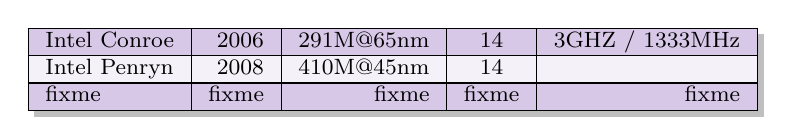
\begin{tikzpicture}
\node[drop shadow,fill=white,inner sep=0pt]
{\rowcolors{1}{RoyalPurple!20}{RoyalPurple!5}
{\footnotesize
\begin{tabular}{|l|r|r|c|r|}
\hline
Intel Conroe & 2006 & 291M@65nm & 14 & 3GHZ / 1333MHz \\
\hline
Intel Penryn & 2008 & 410M@45nm & 14 & \\
\hline
fixme & fixme & fixme & fixme & fixme \\
\hline
\end{tabular}%
}
};
\end{tikzpicture}
\end{center}
\end{frame}

\begin{frame}[t]{AVX + scaling + heterogeneity (FreeBSD 8, Linux 3)}
\begin{block}{Recent Intel}
\begin{itemize}
\item Return of the barrel shifter (and HyperThreading)!
\item Nehalem adds SSE4.2, 2TLB, VT-d, integrates northbridge
\item Quick Path Interconnect on Nehalem-E
\item Sandy Bridge integrates GPU, GMCH, L3, 256-bit AVX
\item Ivy Bridge adds PCIe 3.0, FinFET trigates
\item Haswell adds transactional memory, AVX2, FMA3
\end{itemize}
\end{block}
\vfill
\begin{center}
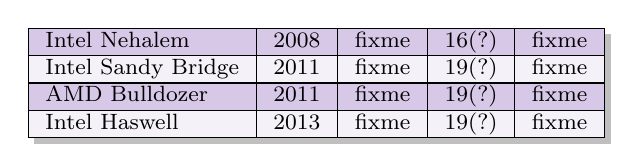
\begin{tikzpicture}
\node[drop shadow,fill=white,inner sep=0pt]
{\rowcolors{1}{RoyalPurple!20}{RoyalPurple!5}
{\footnotesize
\begin{tabular}{|l|r|r|c|r|}
\hline
Intel Nehalem & 2008 & fixme & 16(?) & fixme \\
\hline
Intel Sandy Bridge & 2011 & fixme & 19(?) & fixme \\
\hline
AMD Bulldozer & 2011 & fixme & 19(?) & fixme \\
\hline
Intel Haswell & 2013 & fixme & 19(?) & fixme \\
\hline
\end{tabular}%
}
};
\end{tikzpicture}
\end{center}
\end{frame}

\begin{frame}{Decoding\hfill\tiny{image source: \href{http://realworldtech.com}{Real World Technologies}}}
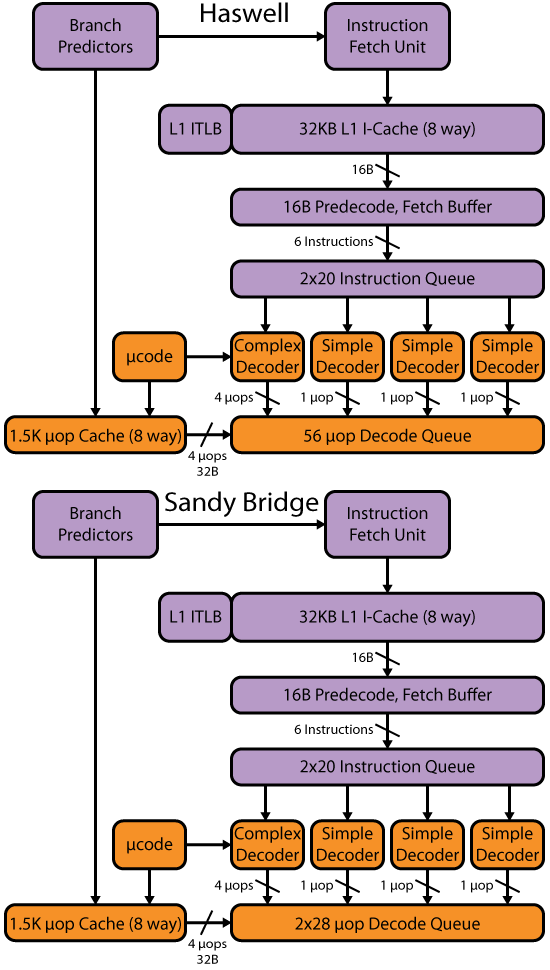
\includegraphics[scale=.49]{images/haswell-1.png}
\end{frame}

\begin{frame}{Schedulers\hfill\tiny{image source: \href{http://realworldtech.com}{Real World Technologies}}}
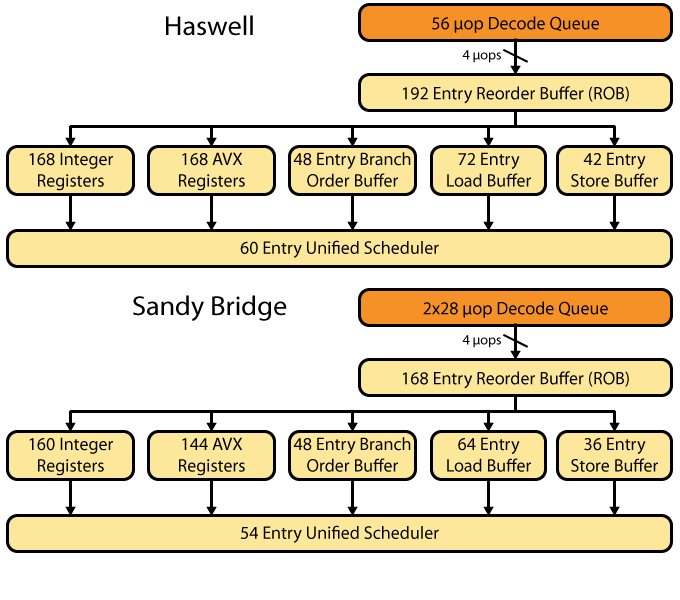
\includegraphics[scale=.42]{images/haswell-2.png}
\end{frame}

\begin{frame}{Execution\hfill\tiny{image source: \href{http://realworldtech.com}{Real World Technologies}}}
\begin{columns}
\begin{column}{.5\textwidth}
\hfill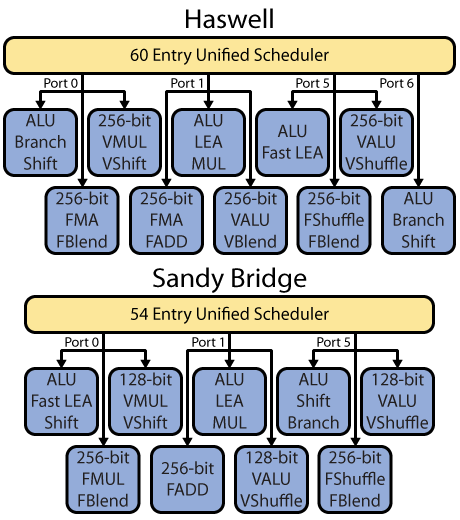
\includegraphics[scale=.45]{images/haswell-3.png}
\end{column}
\end{columns}
\end{frame}

\begin{frame}{Sandy Bridge (2011)\hfill\tiny{image source: \textit{Intel Optimization Manual}}}
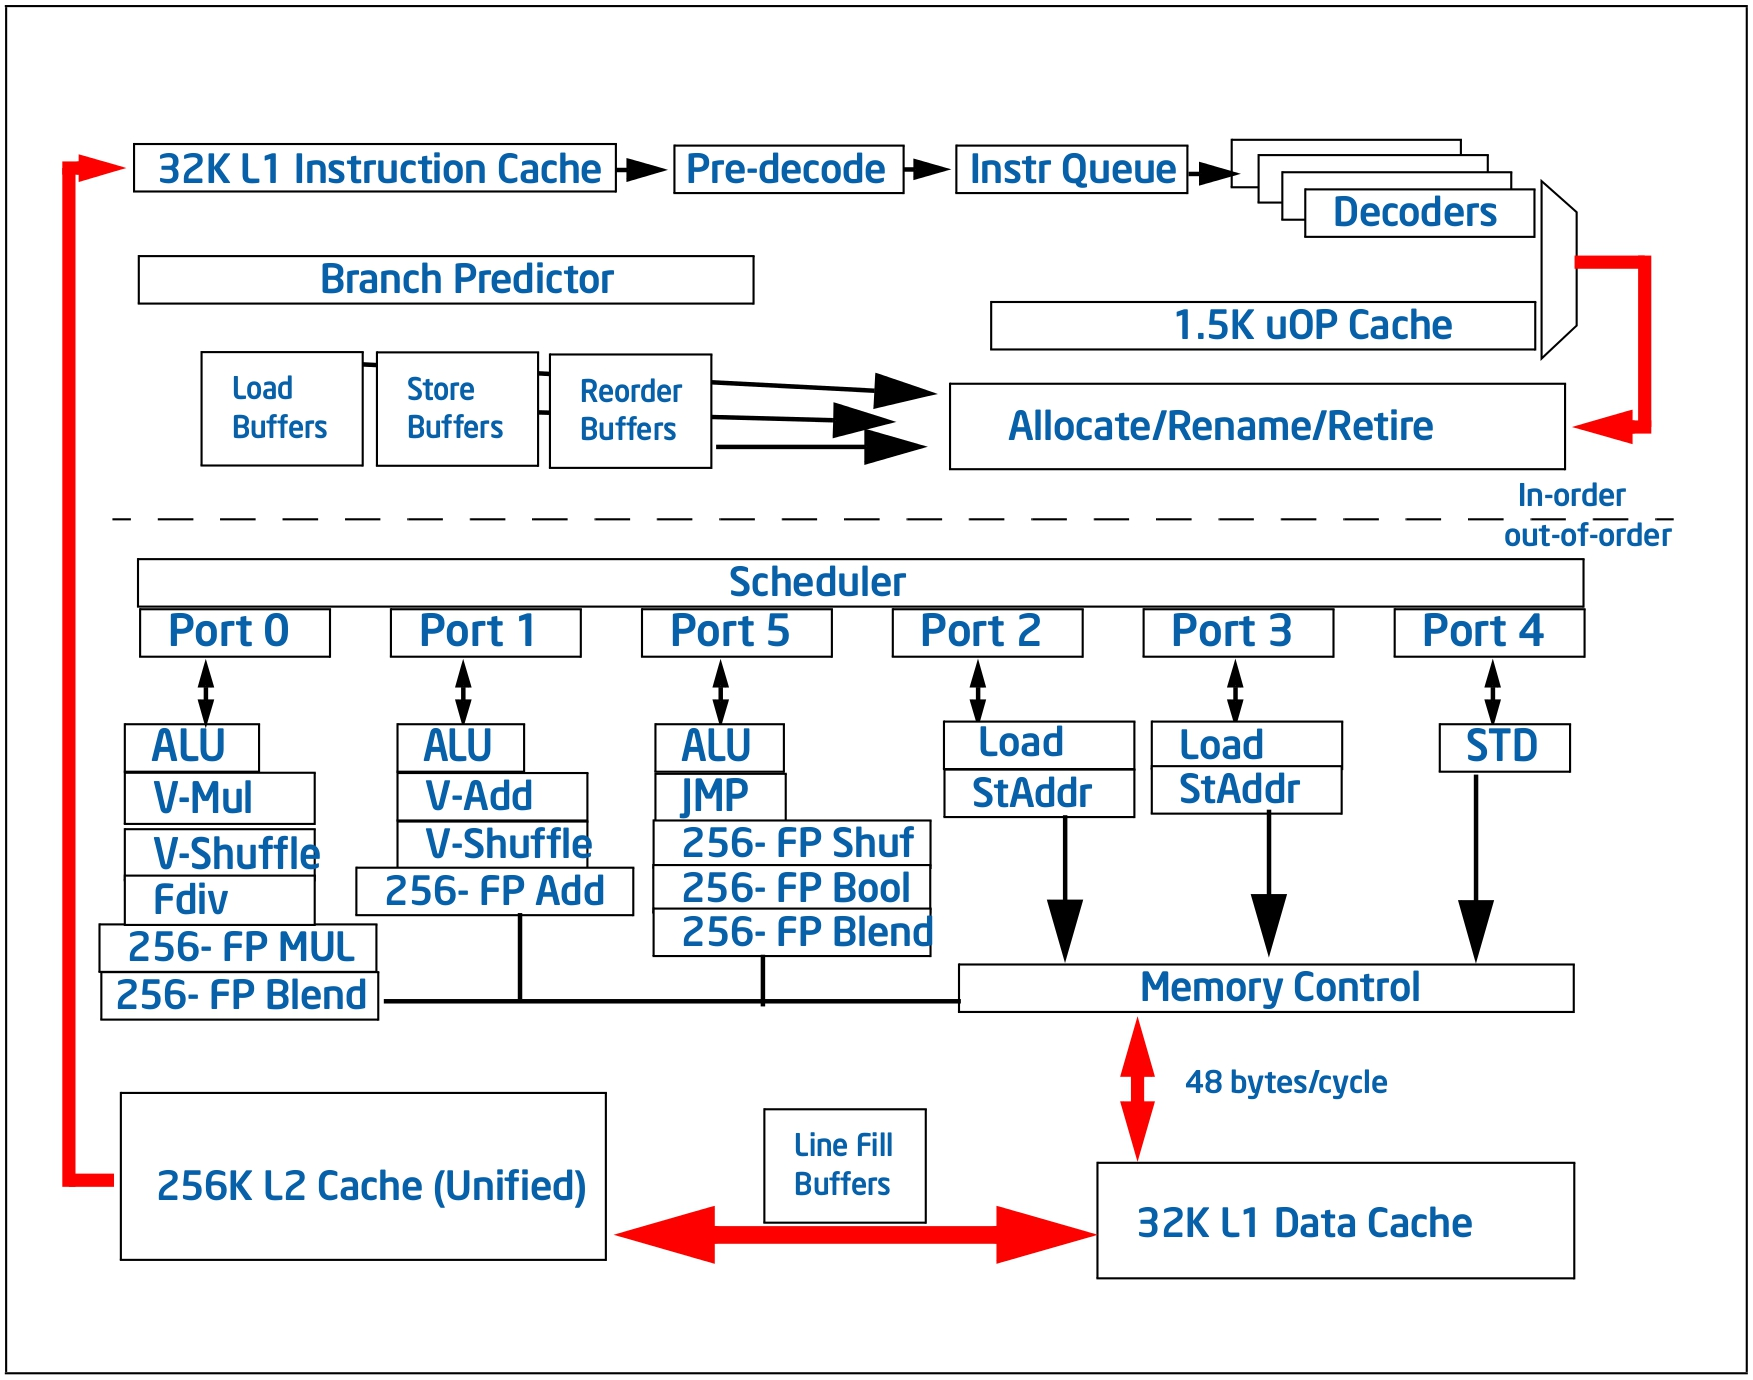
\includegraphics[scale=.175]{images/sandybridge.jpg}
\end{frame}

\begin{frame}{Haswell (2013)\hfill\tiny{image source: \href{http://realworldtech.com}{Real World Technologies}}}
\begin{columns}
\begin{column}{.5\textwidth}
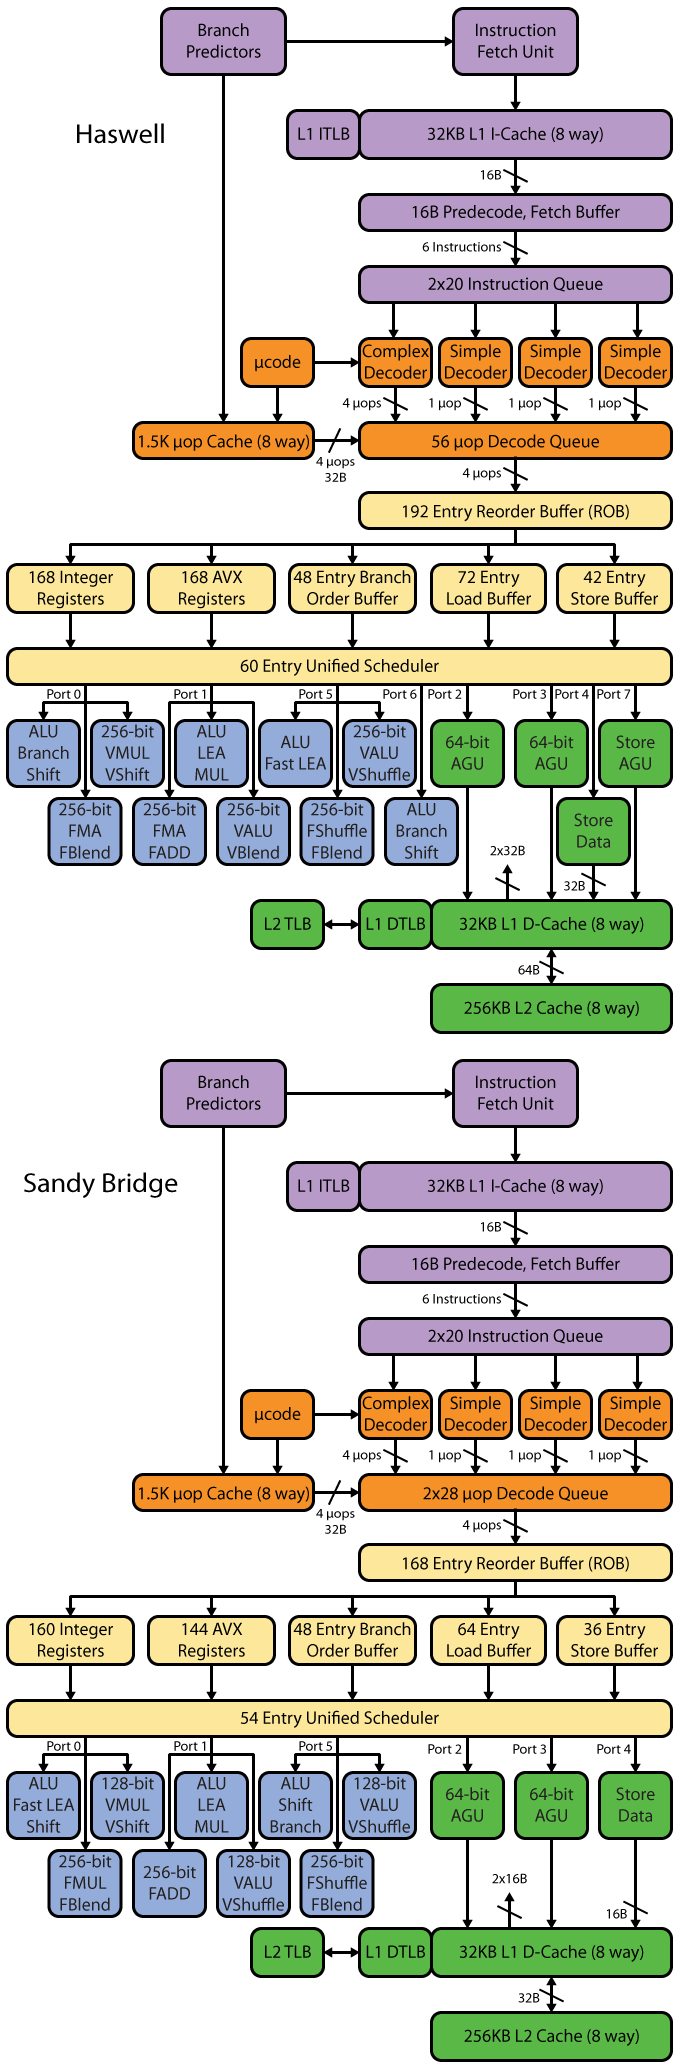
\includegraphics[scale=.225]{images/haswell-5.png}
\end{column}
\end{columns}
\end{frame}

\begin{frame}{Immediate state + instruction store}
\begin{center}
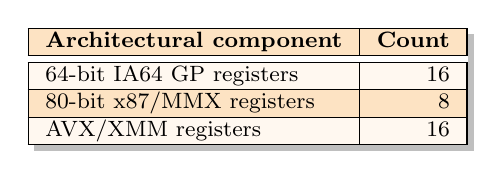
\begin{tikzpicture}
\node[drop shadow,fill=white,inner sep=0pt]
{\rowcolors{1}{BurntOrange!20}{BurntOrange!5}
{\footnotesize
\begin{tabular}{|l|r|}
\hline
\textbf{Architectural component} & \textbf{Count} \\
\hline
\hline
64-bit IA64 GP registers & 16 \\
\hline
80-bit x87/MMX registers & 8 \\
\hline
AVX/XMM registers & 16 \\
\hline
\end{tabular}%
}
};
\end{tikzpicture}

\vspace{.25in}

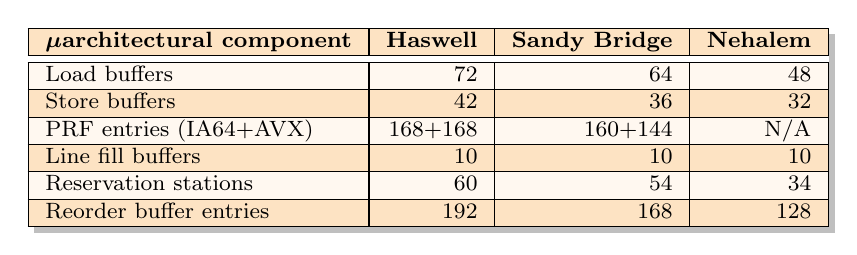
\begin{tikzpicture}
\node[drop shadow,fill=white,inner sep=0pt]
{\rowcolors{1}{BurntOrange!20}{BurntOrange!5}
{\footnotesize
\begin{tabular}{|l|r|r|r|}
\hline
\textbf{$\boldsymbol\mu$architectural component} & \textbf{Haswell} & \textbf{Sandy Bridge} & \textbf{Nehalem} \\
\hline
\hline
Load buffers & 72 & 64 & 48 \\
\hline
Store buffers & 42 & 36 & 32 \\
\hline
PRF entries (IA64+AVX) & 168+168 & 160+144 & N/A \\
\hline
Line fill buffers & 10 & 10 & 10 \\
\hline
Reservation stations & 60 & 54 & 34 \\
\hline
Reorder buffer entries & 192 & 168 & 128 \\
\hline
\end{tabular}%
}
};
\end{tikzpicture}
\end{center}
\begin{itemize}
\item 32KB instruction cache, 16B/\textbf{c}$\implies$48GB/s @ 3GHz
\item 8-way on Sandy Bridge, 4-way on Nehalem
\item 128 4K ITLB entries, 8 large ITLB entries\footnote{7 on Nehalem}
\item MSROM 4$\mu$op/\textbf{c}
\end{itemize}
\end{frame}

\begin{frame}{On-die data store}
The latencies below are best cases (simple address mode, no stalls, no eviction, etc.). MESI details are stored
in L1/L2, while directory details are kept in the LLC (hence the latter's
inclusivity).
\vfill
\begin{columns}
\begin{column}{0.5\textwidth}
\small{
\begin{itemize}
\item 32KB 8-way 64B/line data cache, 4\textbf{c} latency, 2x16B/\textbf{c}
\item Sandy Bridge provides 32B/\textbf{c} L1 load, Haswell 64B/\textbf{c} L1/L2 load and 32B/\textbf{c} L1 store
\item 256KB 8-way 64B/line unified non-inclusive L2, 12\textbf{c} (10\textbf{c} on Nehalem), 32B/\textbf{c}
\item Variable 64B/line unified inclusive L3, 26--31\textbf{c} (35--40\textbf{c} on Nehalem), 32B/\textbf{c}
\item 43\textbf{c}/60\textbf{c} for clean/dirty forward
\end{itemize}
}
\end{column}
\begin{column}{0.5\textwidth}
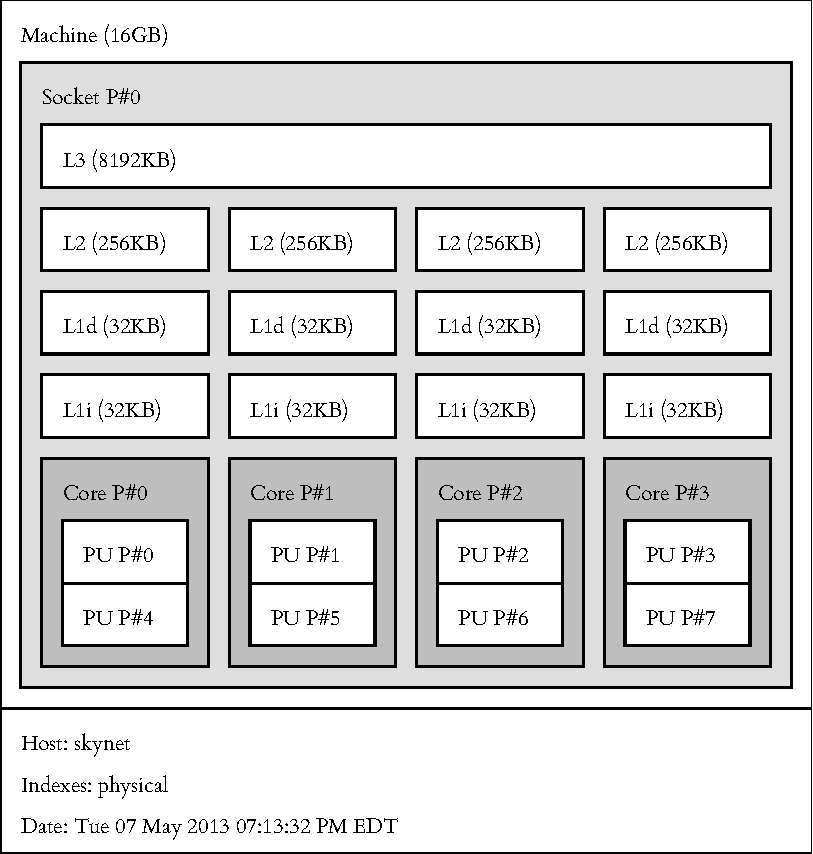
\includegraphics[scale=.4]{images/skynet.pdf}
\end{column}
\end{columns}
\hfill
\tiny{\texttt{lstopo(1)} output}
\end{frame}

\begin{frame}{TLBs and Memory interface}
\begin{itemize}
\item 4-way DTLB translates up to 2 loads/\textbf{c} and 1 store/\textbf{c}
\item DTLB: 64 4KB entries, 32 2MB/4MB entries, 4 1GB entries
\item 4-way unified STLB with 512\footnote{1024 on Haswell} 4KB entries, 7\textbf{c} latency
\item L1: IP-based stride prefetcher, DCU streaming prefetcher
\item L2: Spatial prefetcher, streaming prefetcher
\item Nehalem: 3x 8B DDR3 @ 1.333GT/s (31.992GB/s)
\item Sandy Bridge-E: 4x 8B DDR3 @ 1.6GT/s (51.2GB/s)
\end{itemize}
\textbf{FIXME show PATs/MTRRs, page table hierarchy\ldots}
\end{frame}

\begin{frame}{Instruction set I}
\huge\textbf{FIXME}
\end{frame}

\begin{frame}{Instruction set II}
\huge\textbf{FIXME}
\end{frame}

\begin{frame}{HyperThreading}
\begin{description}
\item[\textbf{Replication}] Registers, renamed RSB, large page ITLB
\item[\textbf{Partition}] Load/store buffers, ROB, small page ITLB
\item[\textbf{Competition}] Reservation stations, cache, DTLB, STLB 
\end{description}
\end{frame}

\begin{frame}{Recommended reading}
\begin{itemize}
\small
\item Bhandarkar and Clark. ``\href{http://dl.acm.org/citation.cfm?id=107003}{Performance from Architecture: Comparing a
RISC and a CISC with Similar Hardware Organization}'' (1991).
\vfill
\item Blem et al. ``\href{http://research.cs.wisc.edu/vertical/papers/2013/hpca13-isa-power-struggles.pdf}{Power Struggles: Revisiting the RISC vs. CISC Debate on
Contemporary ARM and x86 Architectures}'' (2013).
\vfill
\item Michael Thomadakis. ``The Architecture of the Nehalem Processor and
Nehalem-EP SMP Platforms'' (2011).
\vfill
\item Neil Dickson. ``A Simple, Linear-Time Algorithm for x86 Jump Encoding.'' (2011).
\vfill
\item \href{http://www.sandpile.org}{http://www.sandpile.org} and 
\href{http://www.cpu-world.com}{http://www.cpu-world.com}
\vfill
\item \textit{Intel 64 and IA-32 Architectures Instruction Reference}.
\vfill
\item \textit{CUDA Parallel Thread Execution ISA Reference}.
\end{itemize}
\end{frame}

\begin{frame}
``We still have judgment here, that we but teach\\
Bloody instructions, which, being taught, return\\
To plague th' inventor''\\
\hfill---Shakespeare, \textit{Macbeth}
\vfill
``Each day the mythical return Enzian dreamed of seems less possible. Once it
was necessary to know uniforms, insignia, airplane markings, to observe
boundaries. But by now too many choices have been made. The single root lost,
way back there in the May desolation. Each bird has his branch now, and each
one is the Zone.''\\
\hfill---Thomas Pynchon, \textit{Gravity's Rainbow}
\end{frame}

\end{document}
